
\begin{DoxyItemize}
\item \hyperlink{sparse_eigs}{E\-I\-G\-S Sparse Matrix Eigendecomposition}  
\item \hyperlink{sparse_full}{F\-U\-L\-L Convert Sparse Matrix to Full Matrix}  
\item \hyperlink{sparse_sparse}{S\-P\-A\-R\-S\-E Construct a Sparse Matrix}  
\item \hyperlink{sparse_speye}{S\-P\-E\-Y\-E Sparse Identity Matrix}  
\item \hyperlink{sparse_spones}{S\-P\-O\-N\-E\-S Sparse Ones Function}  
\item \hyperlink{sparse_sprand}{S\-P\-R\-A\-N\-D Sparse Uniform Random Matrix}  
\item \hyperlink{sparse_sprandn}{S\-P\-R\-A\-N\-D\-N Sparse Normal Random Matrix}  
\item \hyperlink{sparse_spy}{S\-P\-Y Visualize Sparsity Pattern of a Sparse Matrix}  
\end{DoxyItemize}\hypertarget{sparse_eigs}{}\section{E\-I\-G\-S Sparse Matrix Eigendecomposition}\label{sparse_eigs}
Section\-: \hyperlink{sec_sparse}{Sparse Matrix Support} \hypertarget{vtkwidgets_vtkxyplotwidget_Usage}{}\subsection{Usage}\label{vtkwidgets_vtkxyplotwidget_Usage}
Computes the eigendecomsition of a sparse square matrix. The {\ttfamily eigs} function has several forms. The most general form is \begin{DoxyVerb}  [V,D] = eigs(A,k,sigma)
\end{DoxyVerb}
 where {\ttfamily A} is the matrix to analyze, {\ttfamily k} is the number of eigenvalues to compute and {\ttfamily sigma} determines which eigenvallues to solve for. Valid values for {\ttfamily sigma} are 'lm' -\/ largest magnitude 'sm' -\/ smallest magnitude 'la' -\/ largest algebraic (for real symmetric problems) 'sa' -\/ smallest algebraic (for real symmetric problems) 'be' -\/ both ends (for real symmetric problems) 'lr' -\/ largest real part 'sr' -\/ smallest real part 'li' -\/ largest imaginary part 'si' -\/ smallest imaginary part scalar -\/ find the eigenvalues closest to {\ttfamily sigma}. The returned matrix {\ttfamily V} contains the eigenvectors, and {\ttfamily D} stores the eigenvalues. The related form \begin{DoxyVerb}   d = eigs(A,k,sigma)
\end{DoxyVerb}
 computes only the eigenvalues and not the eigenvectors. If {\ttfamily sigma} is omitted, as in the forms \begin{DoxyVerb}  [V,D] = eigs(A,k)
\end{DoxyVerb}
 and \begin{DoxyVerb}  d = eigs(A,k)
\end{DoxyVerb}
 then {\ttfamily eigs} returns the largest magnitude eigenvalues (and optionally the associated eigenvectors). As an even simpler form, the forms \begin{DoxyVerb}  [V,D] = eigs(A)
\end{DoxyVerb}
 and \begin{DoxyVerb}  d = eigs(A)
\end{DoxyVerb}
 then {\ttfamily eigs} returns the six largest magnitude eigenvalues of {\ttfamily A} and optionally the eigenvectors. The {\ttfamily eigs} function uses A\-R\-P\-A\-C\-K to compute the eigenvectors and/or eigenvalues. Note that due to a limitation in the interface into A\-R\-P\-A\-C\-K from Free\-Mat, the number of eigenvalues that are to be computed must be strictly smaller than the number of columns (or rows) in the matrix. \hypertarget{variables_struct_Example}{}\subsection{Example}\label{variables_struct_Example}
Here is an example of using {\ttfamily eigs} to calculate eigenvalues of a matrix, and a comparison of the results with {\ttfamily eig}


\begin{DoxyVerbInclude}
--> a = sparse(rand(9));
--> eigs(a)

ans = 
   4.1831 +  0.0000i 
   0.3249 -  0.5504i 
   0.3249 +  0.5504i 
   0.5932 -  0.1774i 
   0.5932 +  0.1774i 
  -0.5572 +  0.0000i 

--> eig(full(a))

ans = 
   4.1831 +  0.0000i 
   0.5932 +  0.1774i 
   0.5932 -  0.1774i 
   0.3249 +  0.5504i 
   0.3249 -  0.5504i 
  -0.5572 +  0.0000i 
  -0.1285 +  0.0901i 
  -0.1285 -  0.0901i 
  -0.3219 +  0.0000i 
\end{DoxyVerbInclude}


Next, we exercise some of the variants of {\ttfamily eigs}\-:


\begin{DoxyVerbInclude}
--> eigs(a,4,'sm')

ans = 
  -0.1285 +  0.0901i 
  -0.1285 -  0.0901i 
  -0.3219 +  0.0000i 
  -0.5572 +  0.0000i 

--> eigs(a,4,'lr')

ans = 
   4.1831 +  0.0000i 
   0.5932 +  0.1774i 
   0.5932 -  0.1774i 
   0.3249 +  0.5504i 

--> eigs(a,4,'sr')

ans = 
  -0.5572 +  0.0000i 
  -0.3219 +  0.0000i 
  -0.1285 +  0.0901i 
  -0.1285 -  0.0901i 
\end{DoxyVerbInclude}
 \hypertarget{sparse_full}{}\section{F\-U\-L\-L Convert Sparse Matrix to Full Matrix}\label{sparse_full}
Section\-: \hyperlink{sec_sparse}{Sparse Matrix Support} \hypertarget{vtkwidgets_vtkxyplotwidget_Usage}{}\subsection{Usage}\label{vtkwidgets_vtkxyplotwidget_Usage}
Converts a sparse matrix to a full matrix. The syntax for its use is \begin{DoxyVerb}   y = full(x)
\end{DoxyVerb}
 The type of {\ttfamily x} is preserved. Be careful with the function. As a general rule of thumb, if you can work with the {\ttfamily full} representation of a function, you probably do not need the sparse representation. \hypertarget{variables_struct_Example}{}\subsection{Example}\label{variables_struct_Example}
Here we convert a full matrix to a sparse one, and back again.


\begin{DoxyVerbInclude}
--> a = [1,0,4,2,0;0,0,0,0,0;0,1,0,0,2]

a = 
 1 0 4 2 0 
 0 0 0 0 0 
 0 1 0 0 2 

--> A = sparse(a)

A = 
 1 1 1
 3 2 1
 1 3 4
 1 4 2
 3 5 2
--> full(A)

ans = 
 1 0 4 2 0 
 0 0 0 0 0 
 0 1 0 0 2 
\end{DoxyVerbInclude}
 \hypertarget{sparse_sparse}{}\section{S\-P\-A\-R\-S\-E Construct a Sparse Matrix}\label{sparse_sparse}
Section\-: \hyperlink{sec_sparse}{Sparse Matrix Support} \hypertarget{vtkwidgets_vtkxyplotwidget_Usage}{}\subsection{Usage}\label{vtkwidgets_vtkxyplotwidget_Usage}
Creates a sparse matrix using one of several formats. The first creates a sparse matrix from a full matrix \begin{DoxyVerb}   y = sparse(x).
\end{DoxyVerb}
 The second form creates a sparse matrix containing all zeros that is of the specified size (the sparse equivalent of {\ttfamily zeros}). \begin{DoxyVerb}   y = sparse(m,n)
\end{DoxyVerb}
 where {\ttfamily m} and {\ttfamily n} are integers. Just like the {\ttfamily zeros} function, the sparse matrix returned is of type {\ttfamily float}. The third form constructs a sparse matrix from the I\-J\-V syntax. It has two forms. The first version autosizes the sparse matrix \begin{DoxyVerb}   y = sparse(i,j,v)
\end{DoxyVerb}
 while the second version uses an explicit size specification \begin{DoxyVerb}   y = sparse(i,j,v,m,n)
\end{DoxyVerb}
 \hypertarget{sparse_speye}{}\section{S\-P\-E\-Y\-E Sparse Identity Matrix}\label{sparse_speye}
Section\-: \hyperlink{sec_sparse}{Sparse Matrix Support} \hypertarget{vtkwidgets_vtkxyplotwidget_Usage}{}\subsection{Usage}\label{vtkwidgets_vtkxyplotwidget_Usage}
Creates a sparse identity matrix of the given size. The syntax for its use is \begin{DoxyVerb}  y = speye(m,n)
\end{DoxyVerb}
 which forms an {\ttfamily m x n} sparse matrix with ones on the main diagonal, or \begin{DoxyVerb}  y = speye(n)
\end{DoxyVerb}
 which forms an {\ttfamily n x n} sparse matrix with ones on the main diagonal. The matrix type is a {\ttfamily float} single precision matrix. \hypertarget{variables_struct_Example}{}\subsection{Example}\label{variables_struct_Example}
The following creates a 5000 by 5000 identity matrix, which would be difficult to do using {\ttfamily sparse(eye(5000))} because of the large amount of intermediate storage required.


\begin{DoxyVerbInclude}
--> I = speye(5000);
--> who I
  Variable Name       Type   Flags             Size
              I    double   sparse           [5000x5000]
--> full(I(1:10,1:10))

ans = 
 1 0 0 0 0 0 0 0 0 0 
 0 1 0 0 0 0 0 0 0 0 
 0 0 1 0 0 0 0 0 0 0 
 0 0 0 1 0 0 0 0 0 0 
 0 0 0 0 1 0 0 0 0 0 
 0 0 0 0 0 1 0 0 0 0 
 0 0 0 0 0 0 1 0 0 0 
 0 0 0 0 0 0 0 1 0 0 
 0 0 0 0 0 0 0 0 1 0 
 0 0 0 0 0 0 0 0 0 1 
\end{DoxyVerbInclude}
 \hypertarget{sparse_spones}{}\section{S\-P\-O\-N\-E\-S Sparse Ones Function}\label{sparse_spones}
Section\-: \hyperlink{sec_sparse}{Sparse Matrix Support} \hypertarget{vtkwidgets_vtkxyplotwidget_Usage}{}\subsection{Usage}\label{vtkwidgets_vtkxyplotwidget_Usage}
Returns a sparse {\ttfamily float} matrix with ones where the argument matrix has nonzero values. The general syntax for it is \begin{DoxyVerb}  y = spones(x)
\end{DoxyVerb}
 where {\ttfamily x} is a matrix (it may be full or sparse). The output matrix {\ttfamily y} is the same size as {\ttfamily x}, has type {\ttfamily float}, and contains ones in the nonzero positions of {\ttfamily x}. \hypertarget{variables_matrix_Examples}{}\subsection{Examples}\label{variables_matrix_Examples}
Here are some examples of the {\ttfamily spones} function


\begin{DoxyVerbInclude}
--> a = [1,0,3,0,5;0,0,2,3,0;1,0,0,0,1]

a = 
 1 0 3 0 5 
 0 0 2 3 0 
 1 0 0 0 1 

--> b = spones(a)

b = 
 1 1 1
 1 2 1
 1 3 1
 1 4 1
 1 5 1
--> full(b)

ans = 
 1 1 1 1 1 
 0 0 0 0 0 
 0 0 0 0 0 
\end{DoxyVerbInclude}
 \hypertarget{sparse_sprand}{}\section{S\-P\-R\-A\-N\-D Sparse Uniform Random Matrix}\label{sparse_sprand}
Section\-: \hyperlink{sec_sparse}{Sparse Matrix Support} \hypertarget{vtkwidgets_vtkxyplotwidget_Usage}{}\subsection{Usage}\label{vtkwidgets_vtkxyplotwidget_Usage}
Creates a sparse matrix with uniformly distributed random entries (on \mbox{[}0,1\mbox{]}). The syntax for its use is \begin{DoxyVerb}  y = sprand(x)
\end{DoxyVerb}
 where {\ttfamily x} is a sparse matrix, where {\ttfamily y} is a sparse matrix that has random entries where {\ttfamily x} is nonzero. The second form specifies the size of the matrix and the density \begin{DoxyVerb}  y = sprand(m,n,density)
\end{DoxyVerb}
 where {\ttfamily m} is the number of rows in the output, {\ttfamily n} is the number of columns in the output, and {\ttfamily density} (which is between 0 and 1) is the density of nonzeros in the resulting matrix. Note that for very high densities the actual density of the output matrix may differ from the density you specify. This difference is a result of the way the random entries into the matrix are generated. If you need a very dense random matrix, it is better to generate a full matrix and zero out the entries you do not need. \hypertarget{variables_matrix_Examples}{}\subsection{Examples}\label{variables_matrix_Examples}
Here we seed {\ttfamily sprand} with a full matrix (to demonstrate how the structure of the output is determined by the input matrix when using the first form).


\begin{DoxyVerbInclude}
--> x = [1,0,0;0,0,1;1,0,0]

x = 
 1 0 0 
 0 0 1 
 1 0 0 

--> y = sprand(x)

y = 
 1 1 0.171364
 3 1 0.245464
 2 3 0.0426635
--> full(y)

ans = 
    0.1714         0         0 
         0         0    0.0427 
    0.2455         0         0 
\end{DoxyVerbInclude}


The more generic version with a density of {\ttfamily 0.\-001}. On many systems the following is impossible using full matrices


\begin{DoxyVerbInclude}
--> y = sprand(10000,10000,.001);
--> nnz(y)/10000^2

ans = 
 9.9946e-04 
\end{DoxyVerbInclude}
 \hypertarget{sparse_sprandn}{}\section{S\-P\-R\-A\-N\-D\-N Sparse Normal Random Matrix}\label{sparse_sprandn}
Section\-: \hyperlink{sec_sparse}{Sparse Matrix Support} \hypertarget{vtkwidgets_vtkxyplotwidget_Usage}{}\subsection{Usage}\label{vtkwidgets_vtkxyplotwidget_Usage}
Creates a sparse matrix with normally distributed random entries (mean 0, sigma 1). The syntax for its use is \begin{DoxyVerb}  y = sprandn(x)
\end{DoxyVerb}
 where {\ttfamily x} is a sparse matrix, where {\ttfamily y} is a sparse matrix that has random entries where {\ttfamily x} is nonzero. The second form specifies the size of the matrix and the density \begin{DoxyVerb}  y = sprandn(m,n,density)
\end{DoxyVerb}
 where {\ttfamily m} is the number of rows in the output, {\ttfamily n} is the number of columns in the output, and {\ttfamily density} (which is between 0 and 1) is the density of nonzeros in the resulting matrix. Note that for very high densities the actual density of the output matrix may differ from the density you specify. This difference is a result of the way the random entries into the matrix are generated. If you need a very dense random matrix, it is better to generate a full matrix and zero out the entries you do not need. \hypertarget{variables_matrix_Examples}{}\subsection{Examples}\label{variables_matrix_Examples}
Here we seed {\ttfamily sprandn} with a full matrix (to demonstrate how the structure of the output is determined by the input matrix when using the first form).


\begin{DoxyVerbInclude}
--> x = [1,0,0;0,0,1;1,0,0]

x = 
 1 0 0 
 0 0 1 
 1 0 0 

--> y = sprandn(x)

y = 
 1 1 -0.498012
 3 1 0.813313
 2 3 -1.10282
--> full(y)

ans = 
   -0.4980         0         0 
         0         0   -1.1028 
    0.8133         0         0 
\end{DoxyVerbInclude}


The more generic version with a density of {\ttfamily 0.\-001}. On many systems the following is impossible using full matrices


\begin{DoxyVerbInclude}
--> y = sprandn(10000,10000,.001);
--> nnz(y)/10000^2

ans = 
 9.9952e-04 
\end{DoxyVerbInclude}
 \hypertarget{sparse_spy}{}\section{S\-P\-Y Visualize Sparsity Pattern of a Sparse Matrix}\label{sparse_spy}
Section\-: \hyperlink{sec_sparse}{Sparse Matrix Support} \hypertarget{vtkwidgets_vtkxyplotwidget_Usage}{}\subsection{Usage}\label{vtkwidgets_vtkxyplotwidget_Usage}
Plots the sparsity pattern of a sparse matrix. The syntax for its use is \begin{DoxyVerb}   spy(x)
\end{DoxyVerb}
 which uses a default color and symbol. Alternately, you can use \begin{DoxyVerb}   spy(x,colspec)
\end{DoxyVerb}
 where {\ttfamily colspec} is any valid color and symbol spec accepted by {\ttfamily plot}. \hypertarget{variables_struct_Example}{}\subsection{Example}\label{variables_struct_Example}
First, an example of a random sparse matrix.


\begin{DoxyVerbInclude}
--> y = sprand(1000,1000,.001);
--> spy(y,'ro')
\end{DoxyVerbInclude}


which is shown here  
\begin{DoxyImage}
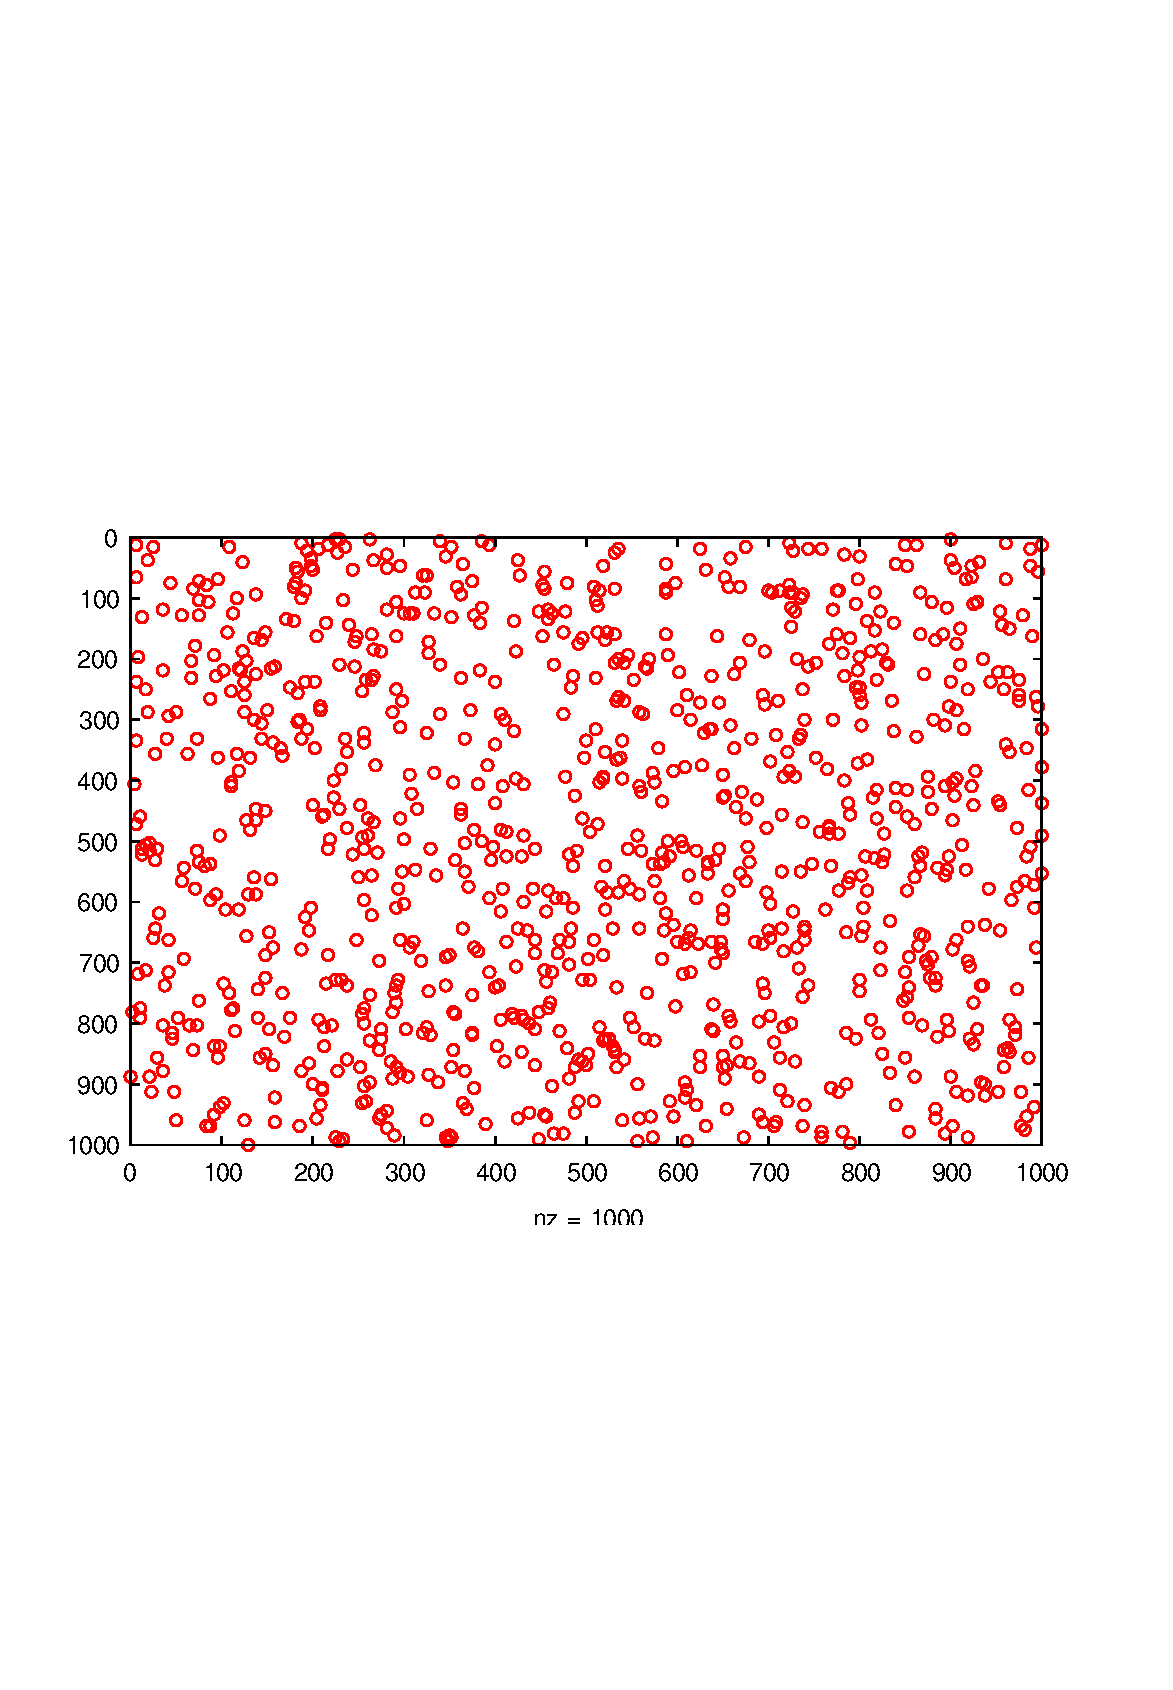
\includegraphics[width=12cm]{spy1}
\caption{spy1}
\end{DoxyImage}
 Here is a sparse matrix with a little more structure. First we build a sparse matrix with block diagonal structure, and then use {\ttfamily spy} to visualize the structure.


\begin{DoxyVerbInclude}
--> A = sparse(1000,1000);
--> for i=1:25; A((1:40) + 40*(i-1),(1:40) + 40*(i-1)) = 1; end;
--> spy(A,'gx')
\end{DoxyVerbInclude}


with the result shown here  
\begin{DoxyImage}
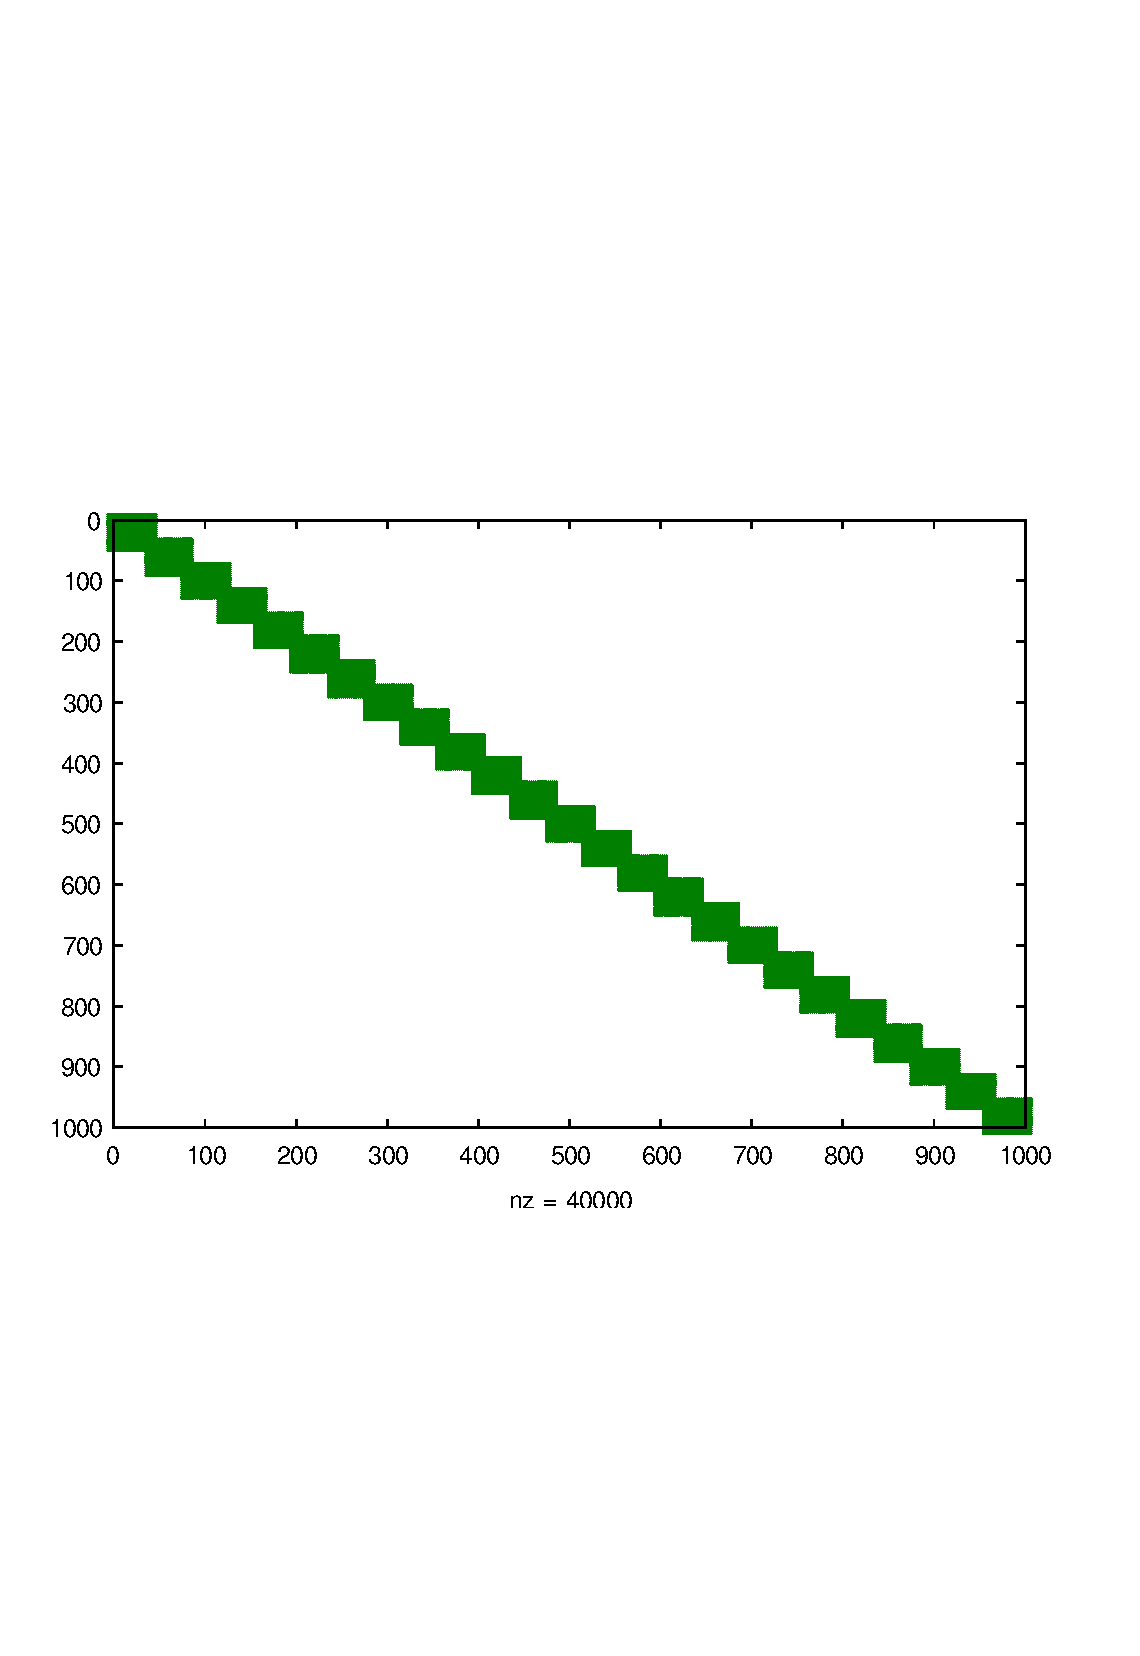
\includegraphics[width=12cm]{spy2}
\caption{spy2}
\end{DoxyImage}
 